%----------------------------------------------------------------------------------------
%	PACKAGES AND THEMES
%----------------------------------------------------------------------------------------
\documentclass[xcolor=dvipsnames]{beamer}
\usetheme{SimplePlus}
\usepackage{hyperref}
\usepackage{graphicx} % Allows including images
\usepackage{booktabs} % Allows the use of \toprule, \midrule and \bottomrule in tables
\usepackage[backend=biber, style=numeric]{biblatex}


\setbeamertemplate{bibliography item}[text]
\addbibresource{urop_surf.bib}

%----------------------------------------------------------------------------------------
%	TITLE PAGE
%----------------------------------------------------------------------------------------

\title[RRT* on an Embedded Optimal Surface]{Improving RRT* for a UAV with Dynamic Constraints in 3 Dimensions Using an Optimal Embedded Surface} % The short title appears at the bottom of every slide, the full title is only on the title page
% \subtitle{Subtitle}

\author[Mike Sutherland] {Mike Sutherland}

\institute[UCI] % Your institution as it will appear on the bottom of every slide, may be shorthand to save space
{
    Department of Mechanical and Aerospace Engineering \\
    University of California, Irvine % Your institution for the title page
}
\date{\today} % Date, can be changed to a custom date


%----------------------------------------------------------------------------------------
%	PRESENTATION SLIDES
%----------------------------------------------------------------------------------------

\begin{document}

\begin{frame}
    % Print the title page as the first slide
    \titlepage
\end{frame}

\begin{frame}{Overview}
    % Throughout your presentation, if you choose to use \section{} and \subsection{} commands, these will automatically be printed on this slide as an overview of your presentation
    \tableofcontents
\end{frame}

\section{Problem And Definitions}

\begin{frame}{Planning In 3-D}
    \begin{itemize}
        \item 3-D planning is expensive
        \item Large search space: $X \times Y \times Z$
        \item Leads to long planning times
    \end{itemize}
\end{frame}

\begin{frame}{What Makes the UAV Problem Unique?}
    \begin{block}{Assumption}
        Lower bounded and simply connected space in $Z$-direction.
    \end{block}
    Physical Interpretation: 
    \begin{itemize}
        \item Terrain (i.e. minimum altitude)
        \item No ceiling (weakly, a very tall ceiling)
        \item A.K.A. Outdoor space
    \end{itemize}
    \begin{figure}
        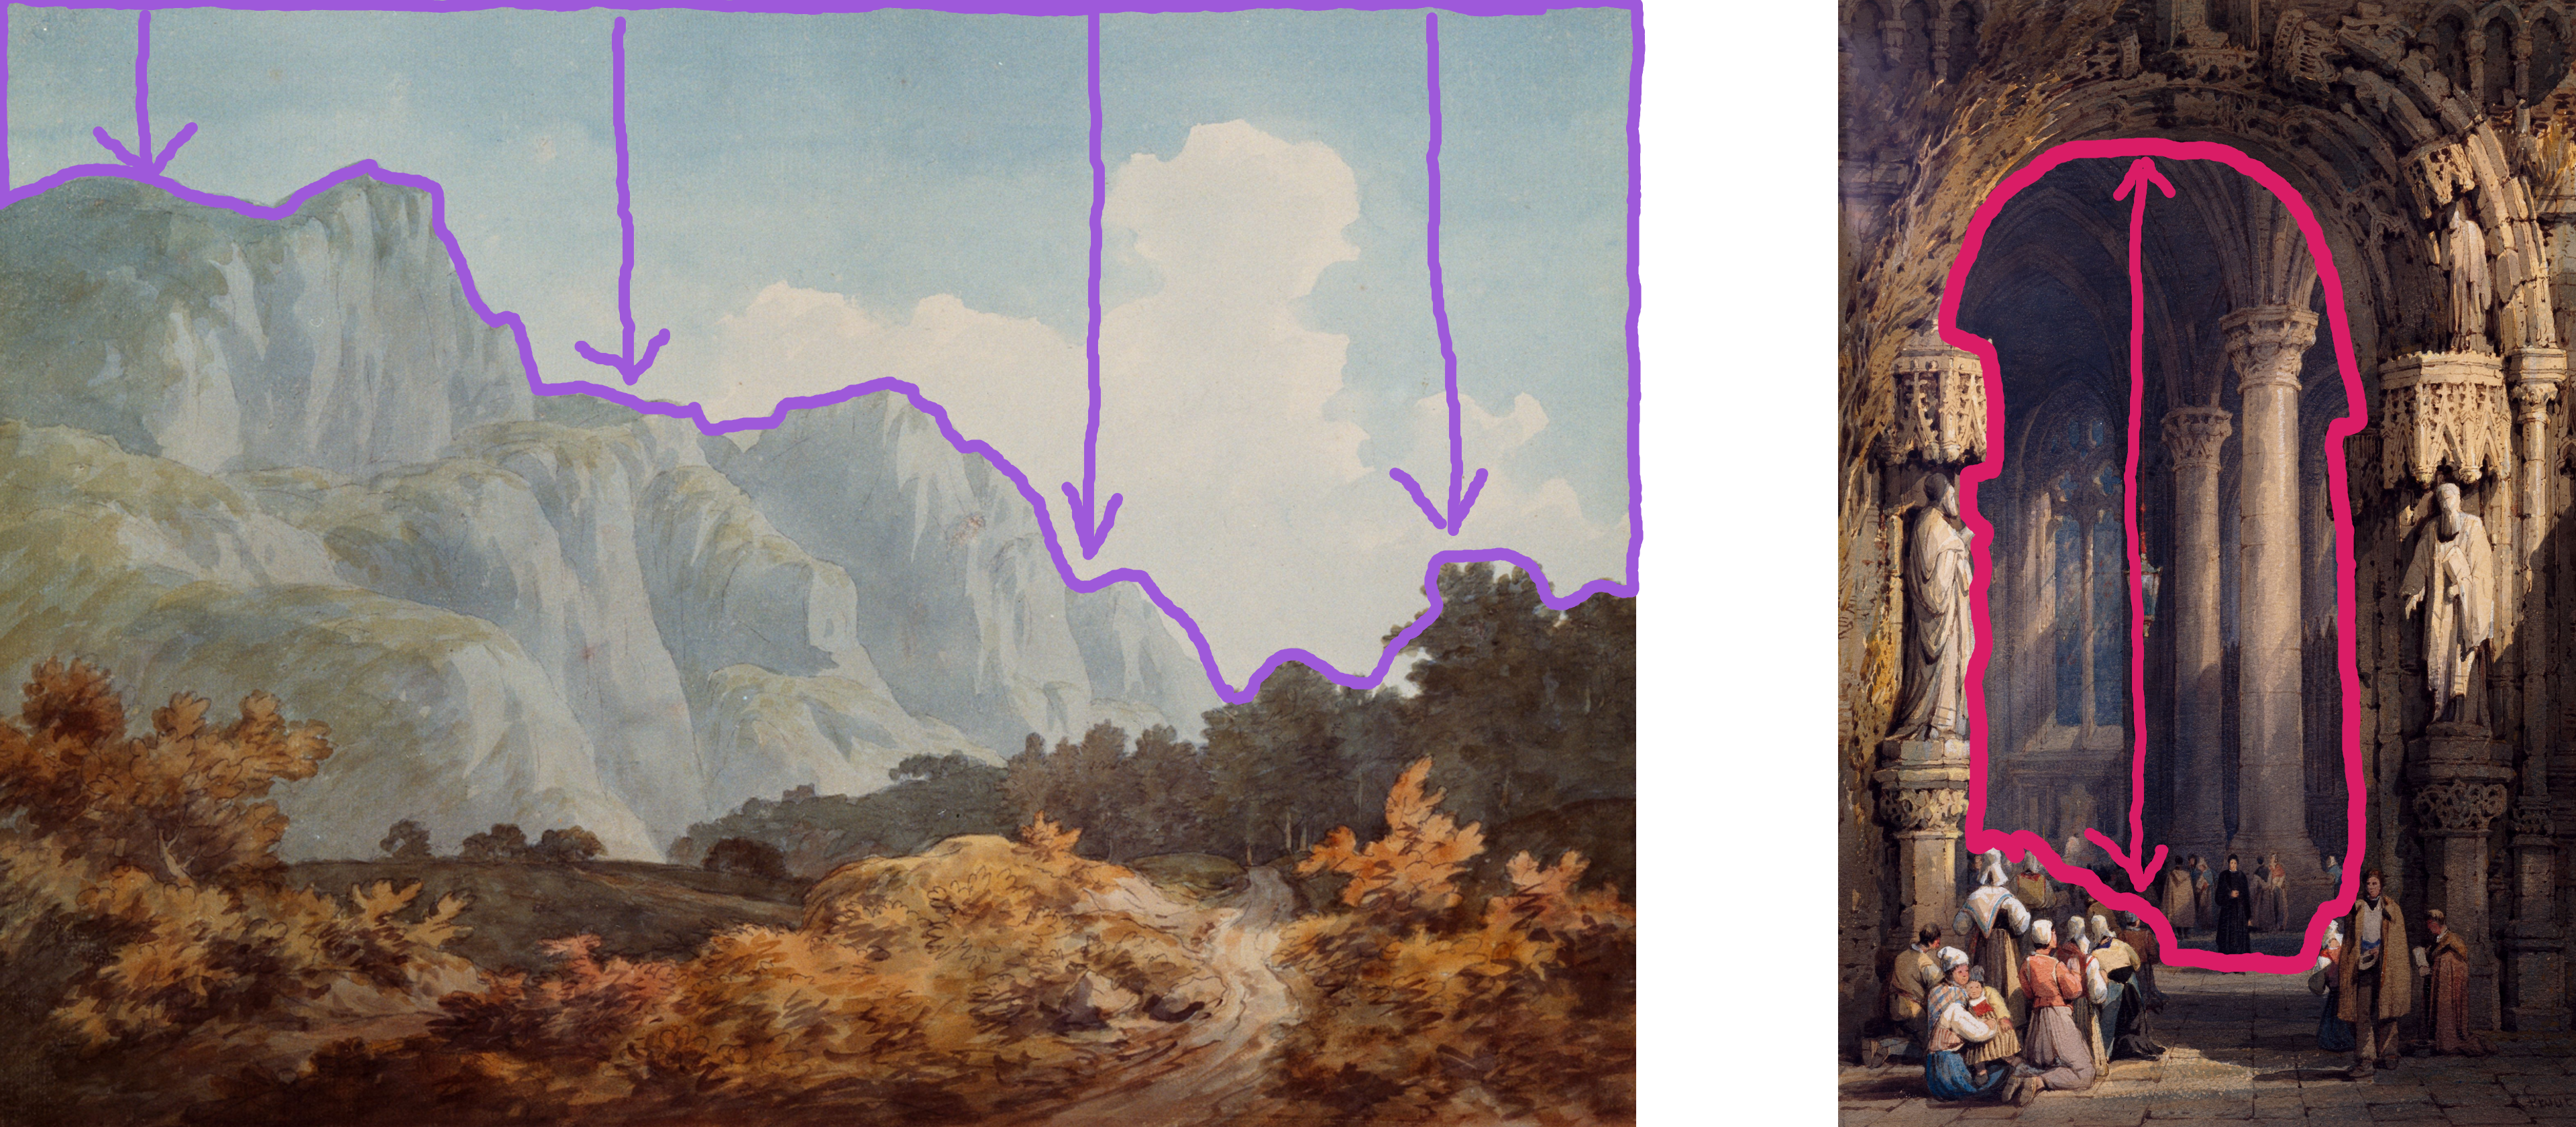
\includegraphics[width=0.7\linewidth]{conf_spaces.png}
        \caption{Left: Valid \cite{smithGlarusSwitzerland1781}; Right: Invalid \cite{proutInteriorCathedral1852}}
    \end{figure}
\end{frame}

\begin{frame}{"Embedded Surface"..?}
    \begin{columns}[c]
        \column{0.5\textwidth}
        We have some constraints:
        \begin{itemize}
        \item Min height
        \item Min climb rate
        \item Min d/dx of climb rate
        \item Safe distance to terrain
        \end{itemize}
        And maybe costs
        \begin{itemize}
        \item Lowest altitude
        \item Waypoints
        \item Desired altitude
        \end{itemize}

        \column{0.4\textwidth}
        \begin{figure}
        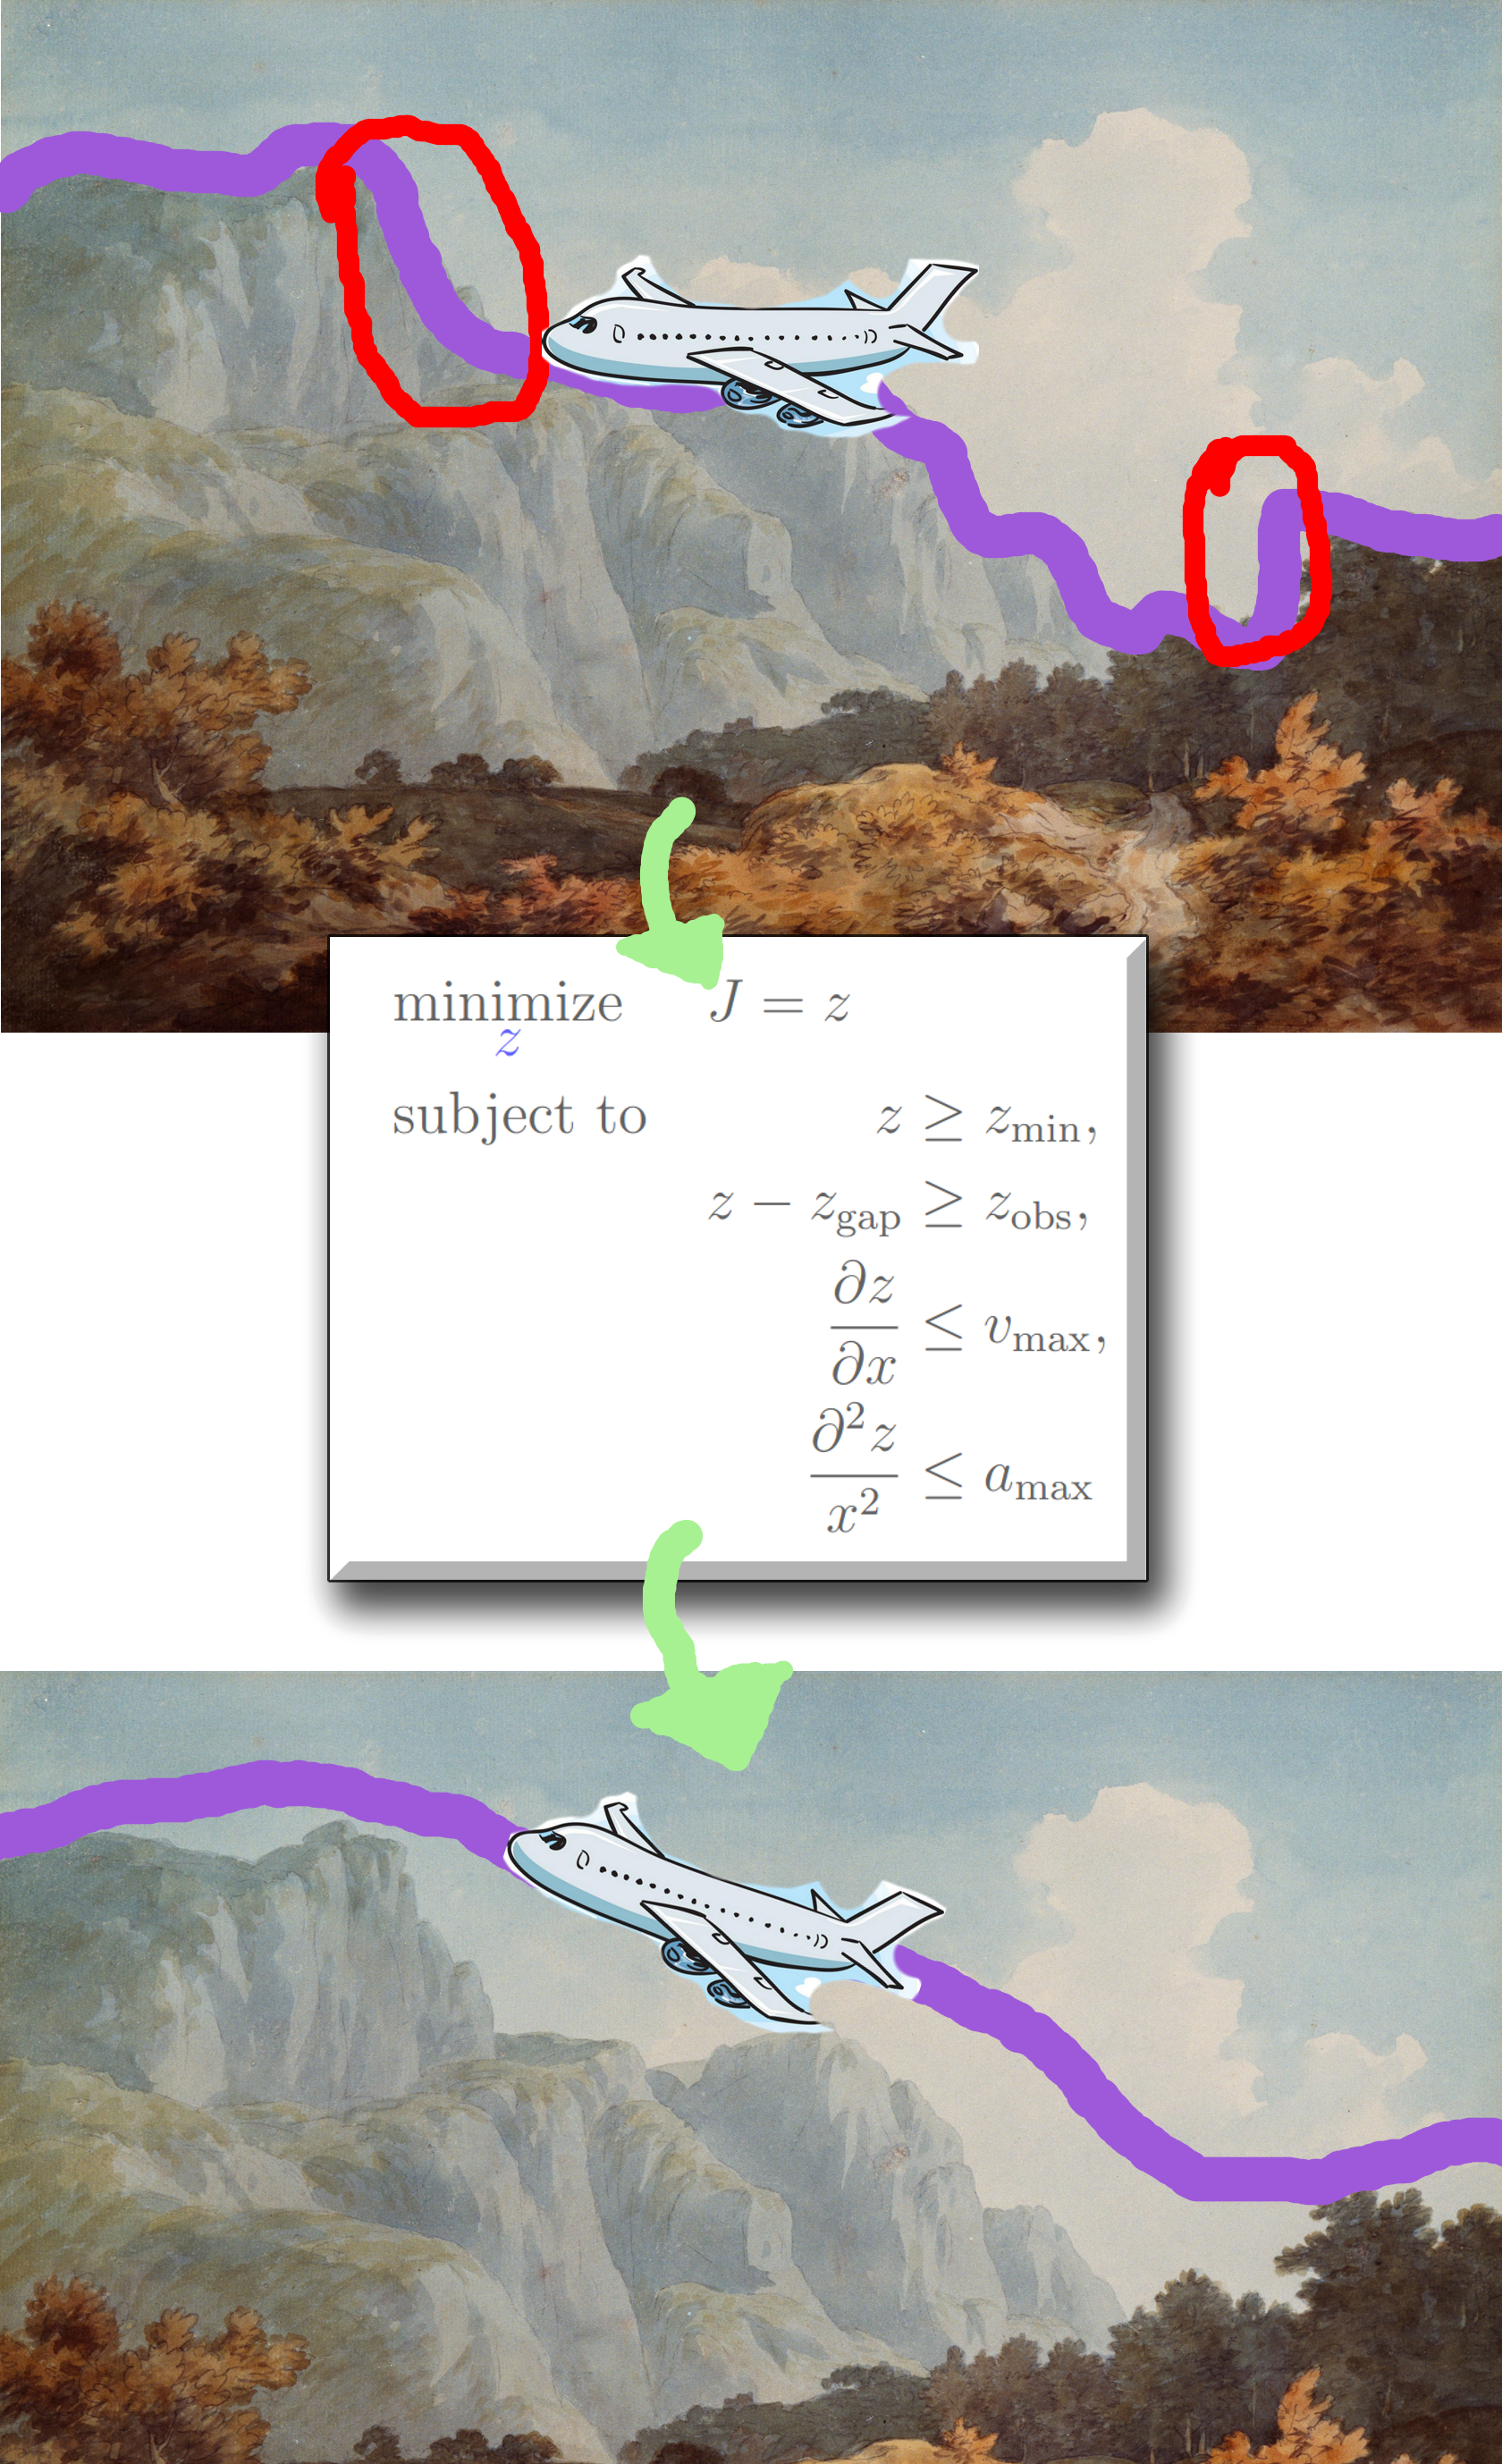
\includegraphics[width=0.9\linewidth]{optim_graphic.png}
        \caption{Optimization}
        \end{figure}

    \end{columns}
\end{frame}


\begin{frame}{References}
    \printbibliography
\end{frame}

\end{document}